
\section{Generazione della Mesh con \texttt{gmsh}}
\label{sec:gmsh}

\subsection{Ruolo della Discretizzazione Spaziale}

Prima di poter risolvere numericamente le equazioni di governo del moto di un fluido, è
necessario discretizzare il dominio fisico continuo in un insieme finito di celle di calcolo.
Questo insieme è la \emph{griglia computazionale} o \emph{mesh}. La qualità della mesh influenza
direttamente sia l'accuratezza della soluzione sia il costo computazionale:
\begin{itemize}
  \item Una griglia \emph{troppo rada} introduce errori di troncamento elevati e non riesce a
    risolvere le strutture fisiche rilevanti (strati limite, onde d'urto, scie);
  \item Una griglia \emph{uniformemente fitta} riduce l'errore ma il costo computazionale cresce
    come $N^d$, con $N$ numero di celle per dimensione e $d$ il numero di dimensioni.
\end{itemize}

La strategia ottimale consiste nel concentrare le celle nelle regioni dove la soluzione varia
rapidamente (grandi gradienti di velocità, pressione o temperatura), mantenendo celle più grandi
nelle zone dove il campo è quasi uniforme. Questa logica è alla base degli strumenti di
raffinamento adattivo disponibili in \textit{gmsh}.

\subsection{Logica di Raffinamento e Algoritmi di Generazione}

La strategia ottimale per la generazione di una griglia computazionale consiste nell'infittire la mesh esclusivamente in quelle regioni in cui i gradienti delle variabili conservative (o fisiche) sono più elevati. Non avrebbe senso, infatti, raffinare la griglia laddove le grandezze si mantengono pressoché costanti (ad esempio nel campo potenziale indisturbato lontano dai corpi): ciò comporterebbe solo un inutile spreco di risorse e potenza computazionale. 

Le zone di forte gradiente coincidono tipicamente con strati limite, onde d'urto, zone di separazione o scie. Per posizionare correttamente l'infittimento, è richiesta un'idea preventiva della fisica del problema e dei fenomeni attesi. Poiché questa conoscenza a priori non è sempre esatta o disponibile, la costruzione della mesh è spesso un processo \emph{iterativo}: si parte con una griglia di primo tentativo, si analizza una soluzione preliminare e si affina la mesh dove i gradienti calcolati risultano maggiori.

Nel software \texttt{gmsh}, la generazione della mesh non strutturata si affida a diversi algoritmi matematici. Uno dei più utilizzati (spesso impostato di default per le mesh 2D) è la \textbf{Triangolazione di Delaunay}. Questo algoritmo collega un insieme di punti nello spazio in modo tale che nessun punto si trovi all'interno della circonferenza circoscritta a un qualsiasi triangolo della mesh. Il vantaggio principale di Delaunay è che tende a massimizzare l'angolo minimo dei triangoli, evitando elementi troppo "schiacciati" (con \textit{aspect ratio} elevato) che potrebbero degradare il condizionamento numerico e l'accuratezza della soluzione.

% ------------------------------------------------------------
\subsection{Il Software \texttt{gmsh}}

\texttt{gmsh} è un generatore di mesh open-source a tre dimensioni con un preprocessore CAD
integrato, un generatore di griglia e un post-processore. I suoi punti di forza nell'ambito di
questo corso sono:
\begin{itemize}
  \item Sintassi scripted tramite file \texttt{.geo}: la geometria e la mesh si definiscono
    programmaticamente, garantendo riproducibilità e facilità di modifica parametrica.
  \item Supporto sia per griglie strutturate (tramite il comando \texttt{Transfinite}) sia per
    griglie non strutturate (triangoli o quadrilateri generati automaticamente).
  \item Strumenti di raffinamento basati su campi scalari di distanza (\textit{Attractor} e
    \textit{Threshold}).
  \item Esportazione nel formato \texttt{.msh} (versione 2.2 nel presente lavoro), direttamente
    leggibile dal codice Fortran sviluppato.
\end{itemize}

% ------------------------------------------------------------
\subsection{Griglie Strutturate e Non Strutturate}
\label{sec:tipi_griglia}

\subsubsection{Griglie Strutturate}

In una griglia strutturata ogni nodo di calcolo si trova all'intersezione di linee coordinate.
Formalmente: \emph{detto $N$ il numero di dimensioni del problema, la griglia è strutturata se
esistono $N$ indici interi tali che scorrere di un'unità su ciascun indice identifichi
univocamente il nodo vicino nella direzione corrispondente.}

\begin{figure}[H]
  \centering
  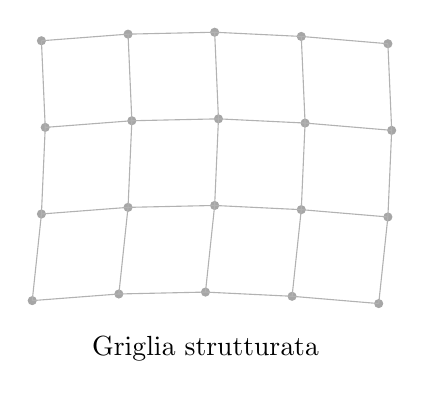
\begin{tikzpicture}[scale=1.1]
    % griglia strutturata 5x4
    \foreach \i in {0,...,4} {
      \foreach \j in {0,...,3} {
        \pgfmathsetmacro{\x}{\i + 0.15*sin(\j*45)}
        \pgfmathsetmacro{\y}{\j + 0.1*sin(\i*50)}
        \fill[gray!70] (\x,\y) circle (1.5pt);
      }
    }
    \foreach \j in {0,...,3} {
      \draw[gray!60, thin]
        ({0+0.15*sin(\j*45)},{\j+0.1*sin(0)})
        -- ({1+0.15*sin(\j*45)},{\j+0.1*sin(50)})
        -- ({2+0.15*sin(\j*45)},{\j+0.1*sin(100)})
        -- ({3+0.15*sin(\j*45)},{\j+0.1*sin(150)})
        -- ({4+0.15*sin(\j*45)},{\j+0.1*sin(200)});
    }
    \foreach \i in {0,...,4} {
      \draw[gray!60, thin]
        ({\i+0.15*sin(0)},{0+0.1*sin(\i*50)})
        -- ({\i+0.15*sin(45)},{1+0.1*sin(\i*50)})
        -- ({\i+0.15*sin(90)},{2+0.1*sin(\i*50)})
        -- ({\i+0.15*sin(135)},{3+0.1*sin(\i*50)});
    }
    \node[below] at (2,-0.3) {Griglia strutturata};
  \end{tikzpicture}
  \hspace{1.5cm}
  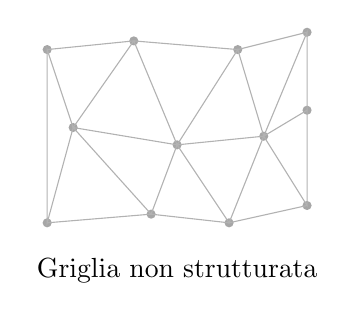
\begin{tikzpicture}[scale=1.1]
    % griglia non strutturata (triangoli casuali)
    \coordinate (A) at (0,0);  \coordinate (B) at (1.2,0.1);
    \coordinate (C) at (2.1,0);\coordinate (D) at (3,0.2);
    \coordinate (E) at (0.3,1.1);\coordinate (F) at (1.5,0.9);
    \coordinate (G) at (2.5,1.0);\coordinate (H) at (3,1.3);
    \coordinate (I) at (0,2);  \coordinate (J) at (1.0,2.1);
    \coordinate (K) at (2.2,2);\coordinate (L) at (3,2.2);
    \foreach \p in {A,B,C,D,E,F,G,H,I,J,K,L}
      \fill[gray!70] (\p) circle (1.5pt);
    \draw[gray!60,thin]
      (A)--(B)--(E)--cycle (B)--(C)--(F)--cycle
      (C)--(D)--(G)--cycle (D)--(H)--(G)--cycle
      (B)--(F)--(E)--cycle (C)--(G)--(F)--cycle
      (E)--(F)--(J)--cycle (F)--(G)--(K)--cycle
      (E)--(J)--(I)--cycle (F)--(K)--(J)--cycle
      (G)--(H)--(L)--cycle (G)--(L)--(K)--cycle
      (D)--(H)--(G)--cycle (A)--(E)--(I)--cycle;
    \node[below] at (1.5,-0.3) {Griglia non strutturata};
  \end{tikzpicture}
  \caption{Schematizzazione di griglia strutturata (sinistra) e non strutturata (destra).}
  \label{fig:tipi_griglia}
\end{figure}

I \textbf{vantaggi} delle griglie strutturate sono:
\begin{itemize}
  \item Non è necessaria una matrice di connettività esplicita: i vicini di ogni cella sono
    identificati incrementando o decrementando gli indici, il che riduce l'occupazione di memoria
    e migliora le prestazioni della cache del processore.
  \item Semplice implementazione di schemi differenziali ad alta precisione.
\end{itemize}

Gli \textbf{svantaggi} sono:
\begin{itemize}
  \item Applicabilità limitata a geometrie relativamente semplici (topologia rettangolare o
    mappabile su di essa);
  \item L'aggiunta di un singolo punto in una zona di interesse richiede l'aggiunta di un'intera
    linea di punti attraverso tutto il dominio, aumentando il costo computazionale globale.
\end{itemize}

\subsubsection{Griglie Non Strutturate}

Nelle griglie non strutturate i nodi non seguono linee coordinate: la loro disposizione nello
spazio è arbitraria e la connettività tra celle deve essere memorizzata esplicitamente in una
matrice di adiacenza. I \textbf{vantaggi} principali sono:
\begin{itemize}
  \item Gestione agevole di geometrie complesse (profili alari, pale di turbina, condotti con
    spigoli vivi);
  \item Possibilità di aggiungere localmente nodi singoli nelle zone di maggiore gradiente senza
    influenzare il resto del dominio;
  \item Generazione quasi-automatica: algoritmi come Delaunay o avanzamento del fronte producono
    griglie di qualità con minima interazione dell'utente.
\end{itemize}

Lo \textbf{svantaggio} principale rispetto alle strutturate è la minore efficienza computazionale
dovuta ai frequenti accessi alla matrice di connettività, che producono un pattern di accesso
alla memoria non sequenziale (\textit{cache-unfriendly}).

% ============================================================
\section{Il File \texttt{.geo} di \texttt{gmsh}}
\label{sec:filegeo}

\texttt{gmsh} legge la geometria e le istruzioni per la mesh da un file di testo con estensione
\texttt{.geo}. La sintassi è procedurale e si svolge gerarchicamente: prima si definiscono i
\emph{punti}, poi le \emph{linee} (rette o curve) che li collegano, poi le \emph{superfici}
delimitate da linee chiuse, e infine le istruzioni per la discretizzazione.

% ------------------------------------------------------------
\subsection{Definizione della Geometria}

\paragraph{Punti.}
Ogni punto è definito con le sue coordinate spaziali e la lunghezza caratteristica locale
$\lc$ desiderata per la mesh in quel punto:
\begin{lstlisting}[style=gmsh, caption={Sintassi del comando \texttt{Point}.}]
Point(i) = {x, y, z, lc};
\end{lstlisting}
dove \texttt{i} è il tag univoco del punto, \texttt{x, y, z} le coordinate (per problemi 2D
si pone \texttt{z~=~0}), e \texttt{lc} la lunghezza caratteristica locale. Specificare un
valore di \texttt{lc} direttamente sul punto è efficace quando ci sono pochi punti; per
domini estesi è preferibile utilizzare i campi di raffinamento descritti nella
Sezione~\ref{sec:campi}.

\paragraph{Linee.}
Una linea retta tra due punti si definisce con:
\begin{lstlisting}[style=gmsh]
Line(i) = {n, m};
\end{lstlisting}
Il verso di percorrenza (da \texttt{n} a \texttt{m}) è rilevante perché determina il segno
delle normali alle superfici. Una curva passante per più punti di controllo è una spline:
\begin{lstlisting}[style=gmsh]
Spline(i) = {n, m, p, q, ...};
\end{lstlisting}
\texttt{gmsh} genera una spline cubica passante per tutti i punti nell'ordine indicato.
Nei file \texttt{.geo} del progetto bump, questa sintassi è usata per descrivere il profilo
del bump sul fondo del condotto.

\paragraph{Linea chiusa e superficie.}
Per definire una superficie è necessario prima creare una \emph{linea chiusa} (loop) che
ne delimiti il contorno:
\begin{lstlisting}[style=gmsh]
Line Loop(i) = {n, m, p, ...};
Plane Surface(j) = {i};
\end{lstlisting}
Le linee nel loop devono formare un percorso chiuso e coerente: se una linea è orientata nel
verso opposto rispetto al percorso, si inserisce il suo tag con segno negativo.

\paragraph{Tag fisici -- condizioni al contorno.}
Il codice CFD riconosce le diverse porzioni del bordo tramite tag numerici assegnati con:
\begin{lstlisting}[style=gmsh]
Physical Surface(tag) = {i, j, ...};   % volume di calcolo
Physical Line(tag)    = {i, j, ...};   % bordi
\end{lstlisting}
La convenzione usata nel codice Fortran è:
\begin{center}
\begin{tabular}{cll}
  \toprule
  Tag & Tipo & Descrizione \\
  \midrule
  1  & \texttt{Physical Surface} & Dominio di calcolo \\
  2  & \texttt{Physical Line}    & Inlet (ingresso) \\
  3  & \texttt{Physical Line}    & Outlet (uscita) \\
  99 & \texttt{Physical Line}    & Parete solida \\
  \bottomrule
\end{tabular}
\end{center}

% ------------------------------------------------------------
\paragraph{\texttt{Transfinite Line} e Progressione Geometrica.}
Quando si impone una distribuzione non uniforme sui lati di una griglia strutturata, è possibile richiedere che la dimensione delle celle segua una \textbf{progressione geometrica}.
\begin{itemize}
  \item \texttt{Using Progression r}: Gli intervalli crescono o decrescono partendo dal nodo iniziale della linea. La legge matematica alla base è una serie geometrica in cui la dimensione di un elemento $h_n$ dipende da quella del precedente tramite un \emph{growth factor} (o ragione) $r$:
  \begin{equation*}
      h_2 = r \cdot h_1 \quad \implies \quad h_n = r^{n-1} h_1
  \end{equation*}
  Si sceglie una serie geometrica per la sua semplicità di calcolo e perché garantisce una transizione fluida e continua tra celle piccole e celle grandi.
  \item \textbf{Inversione della direzione (segno meno)}: Selezionando l'ID della linea con un segno negativo (es. \texttt{-3}), si inverte il verso intrinseco di percorrenza. Di conseguenza, anziché infittirsi all'inizio della linea per poi diradarsi, la mesh partirà rada all'inizio per infittirsi verso la fine dell'elemento.
  \item \texttt{Using Bump r}: Distribuzione simmetrica con addensamento al \emph{centro} della linea. Il parametro $r$ controlla il rapporto tra la dimensione dell'elemento centrale e quella agli estremi.
\end{itemize}

% ------------------------------------------------------------
\subsection{Mesh Non Strutturata: Campi di Raffinamento}
\label{sec:campi}

Per le griglie non strutturate, \texttt{gmsh} offre un potente sistema basato su \emph{campi
scalari} che definiscono la lunghezza caratteristica desiderata in ogni punto del dominio.
La logica è la seguente:

\begin{enumerate}
  \item Si definisce un campo \textbf{Attractor} che calcola la distanza di ogni punto del
    dominio da un insieme di linee (o punti) di riferimento.
  \item Si definisce un campo \textbf{Threshold} che, in funzione della distanza dall'attrattore,
    assegna una lunghezza caratteristica variabile secondo tre zone:
    \begin{itemize}
      \item Zona \emph{vicina} ($d < \texttt{DistMin}$): $\lc = \texttt{LcMin}$ (mesh fitta).
      \item Zona \emph{lontana} ($d > \texttt{DistMax}$): $\lc = \texttt{LcMax}$ (mesh rada).
      \item Zona \emph{di transizione} ($\texttt{DistMin} \le d \le \texttt{DistMax}$):
        $\lc$ varia linearmente tra \texttt{LcMin} e \texttt{LcMax}.
    \end{itemize}
  \item Il campo Threshold è assegnato come \texttt{Background Field}.
\end{enumerate}

\begin{figure}[H]
  \centering
  \begin{tikzpicture}[>=Stealth]
    \begin{axis}[
      width=10cm, height=6cm,
      xlabel={Distanza $d$ dall'attrattore},
      ylabel={Lunghezza caratteristica $\lc$},
      xmin=0, xmax=10,
      ymin=0, ymax=0.65,
      xtick={0,3,7,10},
      xticklabels={$0$,\texttt{DistMin},\texttt{DistMax},$\infty$},
      ytick={0.1,0.5},
      yticklabels={\texttt{LcMin},\texttt{LcMax}},
      axis lines=left,
      grid=major, grid style={gray!20},
    ]
      \addplot[thick, blue!70!black, domain=0:3] {0.1};
      \addplot[thick, blue!70!black, domain=3:7] {0.1 + (0.5-0.1)*(x-3)/(7-3)};
      \addplot[thick, blue!70!black, domain=7:10] {0.5};
      \addplot[dashed, gray] coordinates {(3,0)(3,0.1)};
      \addplot[dashed, gray] coordinates {(7,0)(7,0.5)};
    \end{axis}
  \end{tikzpicture}
  \caption{Andamento della lunghezza caratteristica $\lc$ in funzione della distanza
           dall'attrattore (campo \texttt{Threshold}).}
  \label{fig:threshold}
\end{figure}

La sintassi completa è:
\begin{lstlisting}[style=gmsh, caption={Definizione di Attractor e Threshold in \texttt{gmsh}.}]
// Campo attrattore: calcola la distanza dalle linee indicate
Field[1] = Attractor;
Field[1].EdgesList = {3, 4, 5};  // linee attrattore

// Campo soglia: definisce lc in base alla distanza
Field[2] = Threshold;
Field[2].IField  = 1;       // riferimento al campo Attractor
Field[2].LcMin   = 0.005;   // lc nella zona vicina alla parete
Field[2].LcMax   = 0.05;    // lc nella zona lontana
Field[2].DistMin = 0.05;    // distanza sotto cui si usa LcMin
Field[2].DistMax = 0.15;    // distanza oltre cui si usa LcMax

// Attivazione del campo come background
Background Field = 2;
\end{lstlisting}

È possibile definire più attrattori e più campi Threshold, combinandoli con un campo
\texttt{Min} per prendere il minimo tra diverse regole di raffinamento.

\subsection{Struttura del File \texttt{.msh}: Gli Elementi}

Mentre il file \texttt{.geo} contiene le istruzioni procedurali, il risultato della discretizzazione viene esportato nel formato \texttt{.msh}. Questo file contiene l'elenco dei nodi (coordinate spaziali) e la definizione topologica degli \emph{elementi}. 

È fondamentale comprendere la sintassi con cui \texttt{gmsh} elenca gli elementi per poterli leggere correttamente all'interno del codice Fortran. La sezione degli elementi inizia con la keyword \texttt{\$Elements} seguita dal numero totale di elementi, e si presenta come una lista multi-colonna.

\begin{table}[H]
  \centering
  \caption{Esempio di sintassi degli elementi in un file \texttt{.msh} (versione 2.2).}
  \label{tab:msh_elements}
  \begin{tabular}{cccccc}
    \toprule
    ID Elemento & Tipo & N. Tag & Tag Fisico & Tag Geomet. & Lista Nodi \\
    \midrule
    1807 & 1 & 2 & 3 & 1 & 125 \dots \\
    1808 & 1 & 2 & 3 & 1 & 156 \dots \\
    1809 & 2 & 2 & 1 & 1 & 12 \dots \\
    \bottomrule
  \end{tabular}
\end{table}

Il significato delle colonne è il seguente:
\begin{enumerate}
  \item \textbf{ID Elemento}: Un numero intero progressivo che identifica l'elemento.
  \item \textbf{Tipo}: Specifica la natura geometrica dell'elemento (ad es., \texttt{1} per una linea a 2 nodi, \texttt{2} per un triangolo a 3 nodi, \texttt{3} per un quadrilatero a 4 nodi).
  \item \textbf{Numero di Tag}: Indica quanti tag seguono prima della lista dei nodi (solitamente 2).
  \item \textbf{Tag Fisico}: Il valore assegnato tramite il comando \texttt{Physical Surface} o \texttt{Physical Line} nel file \texttt{.geo} (es. 1 per il dominio, 99 per la parete). Questo è il tag che il solutore CFD utilizza per applicare le corrette condizioni al contorno.
  \item \textbf{Tag Geometrico}: Identifica l'entità geometrica elementare (la linea o la superficie di base) a cui l'elemento appartiene.
  \item \textbf{Lista Nodi}: L'elenco degli ID dei nodi che compongono l'elemento. Il numero di nodi letti dipende dal \emph{Tipo} di elemento definito nella seconda colonna.
\end{enumerate}
% ============================================================